\documentclass{report}

\renewcommand{\thesection}{\arabic{section}}
\usepackage[backend=biber, style=numeric]{biblatex}
\usepackage{indentfirst}
\usepackage{mdframed}
\usepackage{amsmath}
\usepackage{amsthm}
\usepackage{pgfplots}
\usepackage{booktabs}
\usepackage[table,xcdraw]{xcolor}
\usepackage{listings}
\usepackage{color}

\definecolor{pblue}{rgb}{0.13,0.13,1}
\definecolor{pgreen}{rgb}{0,0.5,0}
\definecolor{pred}{rgb}{0.9,0,0}
\definecolor{pgrey}{rgb}{0.46,0.45,0.48}

\usepackage{listings}
\lstset{language=Java,
	showspaces=false,
	showtabs=false,
	breaklines=true,
	showstringspaces=false,
	breakatwhitespace=true,
	commentstyle=\color{pgreen},
	keywordstyle=\color{pblue},
	stringstyle=\color{pred},
	basicstyle=\ttfamily,
	moredelim=[il][\textcolor{pgrey}]{$$},
	moredelim=[is][\textcolor{pgrey}]{\%\%}{\%\%}
}
\addbibresource{complexityAnalysis.bib}
\newtheorem{definition}{Defintion}

\begin{document}
	\title{\textbf{CPT108 Assignment 1:}\\Complexity Analysis}
	\author{Felix Lianto (2362727)\\
			[1cm]{Instructor: Ho Lam}}
	\maketitle
	
\section{Introduction}
The \textit{computational complexity} of an algorithm is defined as the minimum amount of resources needed for an algorithm to solve a computational problem \autocite{vadhanComputationalComplexity2011}. The study behind this is called the \textit{computational complexity theory}. In this area of study, it is most often associated with optimizing the running time and memory space of an algorithm to maximize its efficiency. This report will explore these topics through a basic analysis of common sorting algorithms, which are, 
\begin{itemize}
	\itemsep 0.25pt
	\item Bubble Sort,
	\item Insertion Sort,
	\item Selection Sort,
	\item Merge Sort,
	\item Quick Sort, and
	\item Heap Sort.
\end{itemize}

\underline{This experiment aims to explore:}
\begin{enumerate}
	\item How each sorting algorithms performs with respect to its execution time,
	\item The runtime of each sorting algorithms under certain inputs, and
	\item The memory usage of the sorting algorithms, measured through finding the maximum array size can the Java Virtual Machine (JVM) heap allocate for each sorting algorithm under limited heap size. 
\end{enumerate}

\subsection{Brief Overview of Computational Complexity Analysis}
As mentioned previously, computational complexity can be measured in two dimensions, running time and memory space. Running time of an algorithm, more commonly known as the \textit{time complexity}, is equivalent to the amount of "steps" an algorithm needs to take in order to arrive at an answer \autocite{vadhanComputationalComplexity2011}. In similar fashion, \textit{space complexity} concerns itself with the amount of memory usage an algorithm requires in order to run its code. Both types of resources are measured with \textit{asymptotic notation}, where the amount of "steps" required is represented by a function of its input length \autocite{aroraComputationalComplexityModern2016}. This is to ensure that its performance is language and machine independent, that is, the algorithm will perform similarly when dealing with larger and larger inputs, regardless of the programming language its implemented on, or the machine its working on.

\subsection{Asymptotic Analysis}
As stated before, algorithms can be measured through this universal language of asymptotic notation. These algorithms are commonly grouped together to form \textit{complexity classes}, where given a large enough input, the performance will grow similarly to each other. Figure \ref{compFunc} shows the common orders of complexity that frequently occurs in asymptotic analysis.
\begin{figure}[h]
	\centering
	\begin{mdframed}
		\[
		O(1) < O(\log n) < O(n) < O(n^c) < O(c^n) < O(n!)
		\] \[
		\text{Constant} < \text{Logarithmic} < \text{Linear} < \text{Polynomial} < \text{Exponential} < \text{Factorial}
		\]
	\end{mdframed}
	\caption{Common complexities of asymptotic functions}
	\label{compFunc}
\end{figure}

It is important to emphasize that the asymptotic complexity, regardless if it is time or space, is only a loose estimate of the actual amount of steps required for the algorithm to return successfully. Indeed, some algorithms, even if they share the same complexity class, can still perform better or worse than other algorithms.

To accurately analyze an algorithms' performance, asymptotic notation oftentimes deal with extremes, that is, analyzing the lower and upper bound of a function. These bounds are referred to as the \textit{Big-Oh notation} and the \textit{Big-Omega notation}. Formally, they are defined as follows.
\begin{definition}[Big-Oh Notation \autocite{skienaAlgorithmDesignManual2010}]
	$f(n)$ is a lower bound of $g(n)$ if there exists some constant $c$ and $n_0$ such that for every $n \geq n_0$, $f(n) \leq c \cdot g(n)$. This can be commonly written as $f(n) = O(g(n))$.
\end{definition}
\begin{definition}[Big-Omega Notation \autocite{skienaAlgorithmDesignManual2010}]
	$f(n)$ is an upper bound of $g(n)$ if there exists some constant $c$ and $n_0$ such that for every $n \geq n_0$, $f(n) \geq c \cdot g(n)$. This can be commonly written as $f(n) = \Omega(g(n))$.
\end{definition}

One more important asymptotic notation is the \textit{Big-Theta notation}, which is the intersection of both the Big-Oh and Big-Omega notation, that is, both of the upper and lower bounds of a function can be defined by the same function with different constants. Formally, this is stated as follows.
\begin{definition}[Big-Theta Notation \autocite{skienaAlgorithmDesignManual2010}]
	$f(n)$ is a nice, tight bound of $g(n)$ if there exists some constant $c_1$, $c_2$ and $n_0$ such that for every $n \geq n_0$, $f(n) \leq c_0 \cdot g(n)$ and $f(n) \geq c_1 \cdot g(n)$. This can be expressed as $f(n) = \Theta(g(n))$.
\end{definition}

\subsection{Worst-case, Best-case, and Average-case Time Complexities}
When discussing the efficiency of algorithms with respect to the runtime, it is without a doubt that the type of input can influence the performance of the algorithms. To account for this, the time complexity of these algorithms are split according to its input type, referred to as \textit{worst-case}, \textit{best-case}, and \textit{average-case}. The worst-case time complexity is the maximal function of the number of steps taken for any input of size $n$ \autocite{skienaAlgorithmDesignManual2010}. In contrast, the best-case time complexity is the minimal function given any input of size $n$ \autocite{skienaAlgorithmDesignManual2010}. Finally, between the two extremes, the average-case time complexity, or the \textit{expected time}, is the average function of the number of steps across every input of size $n$ \autocite{skienaAlgorithmDesignManual2010}.

One important to note is that these cases only deal with the input supplied to the algorithm. Oftentimes, these functions would contain unnecessary details about the amount of steps, in which case the asymptotic notation is utilized to describe a loose estimate of the number of steps required. This also implies that for each case, there would be a lower and upper bound that can be specified by asymptotic notation.

\subsection{Time and Space Complexity of Sorting Algorithms}
The focus of this report paper is to investigate the time and space complexity of different sorting algorithms. Thus, before presenting the results of the experiment, a discussion about these sorting algorithms and their theoretical performance will be held in this section. This section will also serve as the hypothesis towards the research questions posed above.

In order to keep this subsection brief, a summary of the time complexities for each case and memory complexity for the sorting algorithms tested will be provided in Table \ref{sumSort}.
\begin{table}[h]
	\centering
	\begin{tabular}{@{}ccccc@{}}
		\toprule
		\multicolumn{1}{|c}{\cellcolor[HTML]{000000}} & \multicolumn{3}{c|}{Time Complexity}          & \multicolumn{1}{c|}{\cellcolor[HTML]{000000}} \\ \midrule
		\multicolumn{1}{c|}{Name of Algorithm}        & Worst-case    & Average-case  & Best-case     & Memory Complexity                             \\ \midrule
		\multicolumn{1}{c|}{Bubble Sort}              & $O(n^2)$      & $O(n^2)$      & $O(n)$        & $O(1)$                                        \\
		\multicolumn{1}{c|}{Insertion Sort}           & $O(n^2)$      & $O(n^2)$      & $O(n)$        & $O(1)$                                        \\
		\multicolumn{1}{c|}{Selection Sort}           & $O(n^2)$      & $O(n^2)$      & $O(n^2)$      & $O(1)$                                        \\
		\multicolumn{1}{c|}{Merge Sort}               & $O(n \log n)$ & $O(n \log n)$ & $O(n \log n)$ & $O(n)$                                        \\
		\multicolumn{1}{c|}{Quick Sort}               & $O(n^2)$      & $O(n \log n)$ & $O(n \log n)$ & $O(1)$                                        \\
		\multicolumn{1}{c|}{Heap Sort}                & $O(n \log n)$ & $O(n \log n)$ & $O(n \log n)$ & $O(1)$                                        \\ \bottomrule
	\end{tabular}
	\caption{Summary of the performance of sorting algorithms \autocite{cormenIntroductionAlgorithms2022}}
	\label{sumSort}
\end{table}

From this table, it is expected that for some random integer array input, the performance would follow the average-case column. That is, Merge Sort, Quick Sort, and Heap Sort would outperform Bubble Sort, Insertion Sort, and Selection Sort. For the worst-case and best-case columns, it will depend on what inputs are inserted into each function. However, differences in time performance between Selection Sort, Merge Sort, and Heap Sort, should not exist, as both their worst-case and best-case time complexity are equal. In other words, these algorithms perform independent of the data supplied.

For Bubble Sort and Insertion Sort, it is expected that their best-cases would be inputs already sorted in ascending order, whilst their worst-cases are inputs sorted in descending order. Furthermore, Merge Sort should see its worst-case performance when either the input is sorted in ascending or descending order. This happens because the algorithm will pick the smallest and biggest pivot every time, thus the list division will always be unequal. Thus, the function will recurse on the same left and right lists twice, thus the $O(n^2)$ time complexity.

Finally, based on the memory complexity column, it is expected that Merge Sort will only sort a small sized integer array before running out of memory, compared to the other sorting algorithms.

\section{Experimental Setup and Procedure}
This experiment will be conducted through the Java Programming Language, where the code will be written and executed in the Eclipse IDE for Java Developers.
The implemented code is written in Java 22, and utilizes 3 built-in classes from the \lstinline|java.util| package. Namely, \lstinline|ArrayList|, \lstinline|Collections|, and \lstinline|Random|.

The script responsible for generating the input data to be tested upon is written by the author themselves, utilizing the \lstinline|Random| class to generate the random numbers, and \lstinline|ArrayList| to store. In some cases, the \lstinline|Collections| class was also used to conveniently sort the generated numbers for the special inputs where the array is already sorted in ascending and descending orders. To ensure the array is deterministic so that for each run of the sorting algorithms operate on the same array, a seed equal to the length of the array was supplied. This way, the generated arrays all have the same elements to ensure no sorting algorithms got an easier array to work with, leading to faster runtime than average. 

Generating the array itself involved a \lstinline|for| loop to generate a random number, then appending it to an initialized \lstinline|ArrayList| object that would be outputted as the resulting random integer array.

The sorting algorithms implemented for testing have all been adapted from the code snippets found on Wikipedia. Links to these algorithms can be found in the documentation of the functions within the source code itself. \\

To measure the execution runtime of the algorithms, the function \lstinline|executionTime| records the program runtime before and after the sorting algorithm is executed. Then, the algorithm's execution time is calculated by taking the difference between the end and start time. This runtime is then printed along with the length of the array divided by $1000$. This is run $20$ times in a \lstinline|for| loop, and the resulting length and algorithm runtime is recorded in a 2D graph as shown in the results section below.

In relation to measuring the memory usage, a binary search approach was implemented to find an approximate maximum array size. Since either a process can crash due to an out-of-memory error or not, and there is a certain cutoff point between when that happens, the binary search method is applicable for solving this problem. A two-pointers approach was taken along with a \lstinline|while| loop to test the midpoint length of the two pointers' array length. To test if an out-of-memory exception would occur, a \lstinline|try-catch| loop was implemented to catch these exceptions and limit the maximum array length to that of the midpoint minus one. Otherwise, the program would limit the lower bound instead to the midpoint plus one.

This loop will repeat until the lower pointer exceeds the higher pointer, in which case it will return the last array length that didn't result in a program crash, which would be our maximum array length. This maximized result is then recorded on a bar graph, to be compared with the maximum array length that the other sorting algorithms require as well. This can be seen in the following section too.

The source code utilized for this experiment can be found in the ZIP file where this report file is located. The source code has been given brief documentations on the details of the algorithms themselves, as well as any further explanation for measuring the execution time and the maximum array size.

\section{Results}

\subsection{Time Performance of Random Integers}
The first aim of the experiment is to compare the runtime performance of each of the sorting algorithms. The comparison will be categorized based on the input array, one consisting of thousands of integers and the other comprising tens of integers.

\subsubsection{Large Array Input}
 This section examines the performance when the array contains thousands of integers. Figure \ref{bigFig} shows the resulting runtime of the 6 sorting algorithms. From the figure, it is apparent that Bubble Sort performed the worst, taking almost triple the time to sort large amounts of integers compared to the second worst. Moreover, it can also be seen that Merge Sort, Quick Sort, and Heap Sort all performed nearly instantaneously, taking no more than $30$ milliseconds to sort thousands of integers.
\begin{figure}
	\centering
	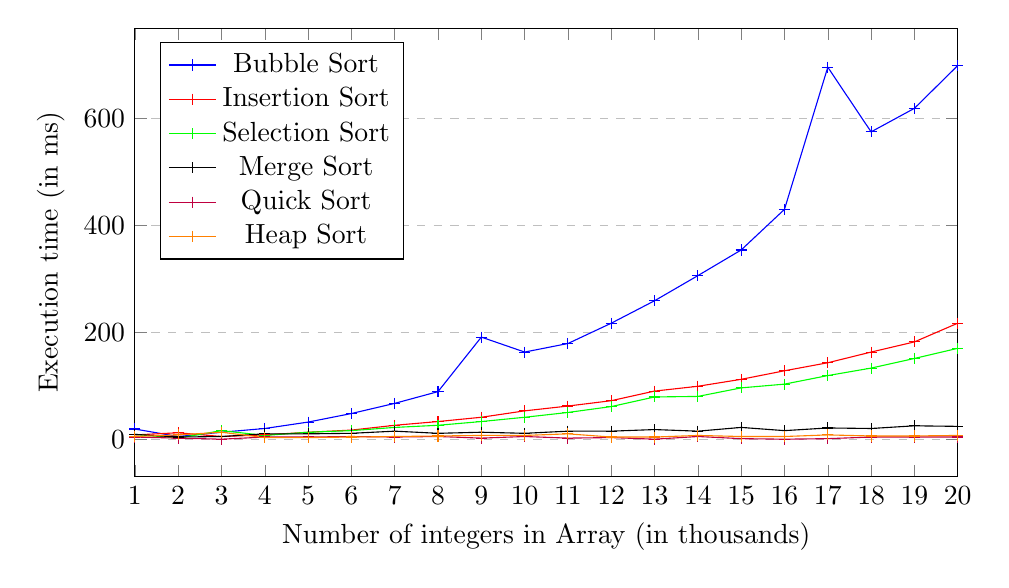
\begin{tikzpicture}
		\begin{axis}[
			xlabel={Number of integers in Array (in thousands)},
			ylabel={Execution time (in ms)},
			x=0.55cm,
			xmin=1, xmax=20,
			xtick={1, 2, 3, 4, 5, 6, 7, 8, 9, 10, 11, 12, 13, 14, 15, 16, 17, 18, 19, 20},
			ymajorgrids=true,
			grid style=dashed,
			legend pos=north west
			]
			
			\addplot[
			color=blue,
			mark=+,
			] 
			coordinates { (1,19)(2,5)(3,13)(4,20)(5,32)(6,48)(7,67)(8,89)(9,191)(10,163)(11,179)(12,217)(13,259)(14,306)(15,354)(16,430)(17,696)(18,575)(19,619)(20,699)};
			
			\addplot[
			color=red,
			mark=+,
			] 
			coordinates { (1,8)(2,12)(3,5)(4,8)(5,13)(6,17)(7,26)(8,33)(9,41)(10,53)(11,62)(12,72)(13,90)(14,99)(15,112)(16,128)(17,143)(18,163)(19,182)(20,217)};
			
			\addplot[
			color=green,
			mark=+,
			] 
			coordinates { (1,9)(2,2)(3,16)(4,7)(5,13)(6,16)(7,22)(8,26)(9,33)(10,41)(11,50)(12,61)(13,79)(14,80)(15,96)(16,103)(17,119)(18,133)(19,151)(20,170)};
			
			\addplot[
			color=black,
			mark=+,
			] 
			coordinates { (1,9)(2,4)(3,5)(4,10)(5,10)(6,11)(7,15)(8,11)(9,13)(10,11)(11,15)(12,15)(13,18)(14,15)(15,22)(16,16)(17,21)(18,20)(19,25)(20,24)};
			
			\addplot[
			color=purple,
			mark=+,
			] 
			coordinates { (1,4)(2,2)(3,0)(4,4)(5,4)(6,5)(7,4)(8,5)(9,2)(10,5)(11,2)(12,3)(13,0)(14,5)(15,1)(16,0)(17,1)(18,4)(19,4)(20,4)};
			
			\addplot[
			color=orange,
			mark=+,
			] 
			coordinates { (1,5)(2,8)(3,13)(4,3)(5,3)(6,4)(7,5)(8,6)(9,7)(10,7)(11,10)(12,4)(13,4)(14,7)(15,5)(16,5)(17,8)(18,6)(19,6)(20,7)};
			\legend{Bubble Sort, Insertion Sort, Selection Sort, Merge Sort, Quick Sort, Heap Sort}
		\end{axis}
	\end{tikzpicture}
	\caption{Execution time of the sorting algorithms with large amounts of random numbers}
	\label{bigFig}
\end{figure}

\subsubsection{Small Array Input}
In contrast to the previous section, this paragraph will focus on small sized arrays. Specifically, arrays of size $5n$ where $0 < n \leq 5$. Figure \ref{smallFig} provides the data for the execution time of the sorting algorithms. From the figure, it is apparent that no definitive trend emerged from any of the sorting algorithms when working with arrays in a small size. Although there are still differences in performance, the overall benefit in speed is inconsequential when measuring in nanoseconds.
\begin{figure}
	\centering
	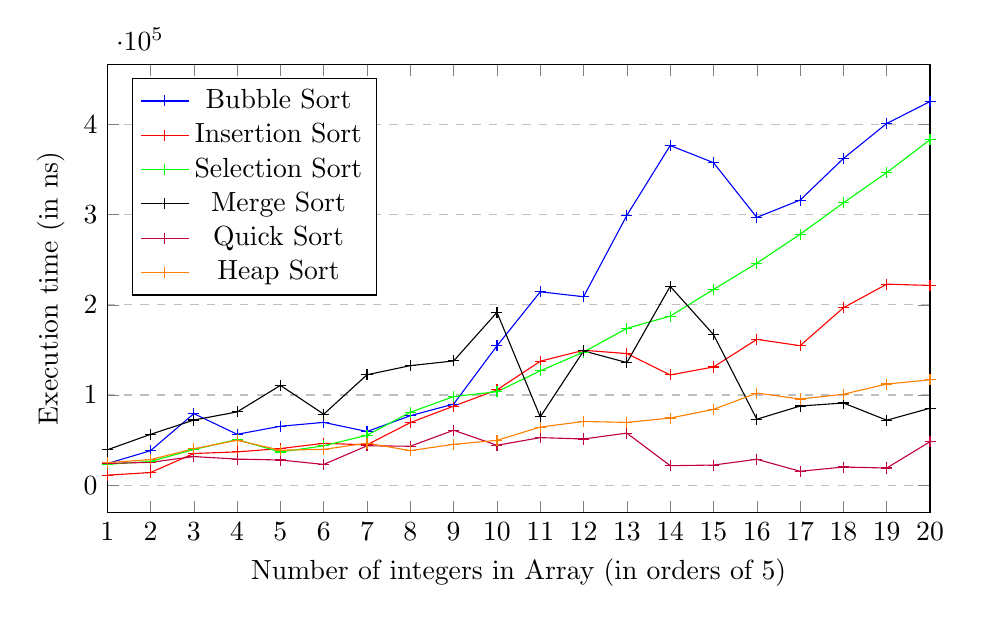
\begin{tikzpicture}
		\begin{axis}[
			xlabel={Number of integers in Array (in orders of 5)},
			ylabel={Execution time (in ns)},
			x=0.55cm,
			xmin=1, xmax=20,
			xtick={1, 2, 3, 4, 5, 6, 7, 8, 9, 10, 11, 12, 13, 14, 15, 16, 17, 18, 19, 20},
			ymajorgrids=true,
			grid style=dashed,
			legend pos=north west
			]
			
			\addplot[
			color=blue,
			mark=+,
			] 
			coordinates { (1,24000)(2,38300)(3,79400)(4,56500)(5,65400)(6,69700)(7,59600)(8,77100)(9,90000)(10,154500)(11,214400)(12,209000)(13,299200)(14,376600)(15,357600)(16,296900)(17,316100)(18,362200)(19,401000)(20,425300)};
			
			\addplot[
			color=red,
			mark=+,
			] 
			coordinates { (1,11200)(2,14100)(3,35200)(4,37000)(5,40700)(6,46500)(7,44800)(8,69500)(9,87700)(10,105700)(11,137500)(12,149600)(13,146000)(14,122300)(15,131100)(16,161700)(17,154700)(18,196800)(19,222900)(20,221500)};
			
			\addplot[
			color=green,
			mark=+,
			] 
			coordinates { (1,23200)(2,26400)(3,39600)(4,50700)(5,36900)(6,43700)(7,55500)(8,80900)(9,98300)(10,103700)(11,126800)(12,147600)(13,173900)(14,187500)(15,217000)(16,246200)(17,278200)(18,313000)(19,346600)(20,383000)};
			
			\addplot[
			color=black,
			mark=+,
			] 
			coordinates { (1,39200)(2,56400)(3,72300)(4,81300)(5,110700)(6,78800)(7,122500)(8,132600)(9,137800)(10,191600)(11,75800)(12,148900)(13,136000)(14,220500)(15,167000)(16,73200)(17,87800)(18,91200)(19,72100)(20,85400)};
			
			\addplot[
			color=purple,
			mark=+,
			] 
			coordinates { (1,24200)(2,25400)(3,31800)(4,29000)(5,28000)(6,23100)(7,43700)(8,43300)(9,61000)(10,44300)(11,52800)(12,51300)(13,57800)(14,21700)(15,22400)(16,28800)(17,15500)(18,20200)(19,19100)(20,48300)};
			
			\addplot[
			color=orange,
			mark=+,
			] 
			coordinates { (1,25100)(2,28400)(3,40500)(4,49800)(5,38900)(6,39800)(7,46700)(8,38400)(9,45400)(10,49800)(11,64500)(12,70700)(13,69700)(14,74500)(15,84100)(16,102200)(17,95600)(18,100900)(19,112200)(20,116900)};
			\legend{Bubble Sort, Insertion Sort, Selection Sort, Merge Sort, Quick Sort, Heap Sort}
		\end{axis}
	\end{tikzpicture}
	\caption{Execution time of the sorting algorithms with small amounts of random numbers}
	\label{smallFig}
\end{figure}

\subsection{Time Performance of Certain Inputs}
The next research question to address concerns the runtime performance of different sorting algorithms working on some special inputs. This subsection has been differentiated into 3 segments, each focusing on a special type of random numbers input.

\subsubsection{Random Ascending Integers}
This part will explore the execution time of sorting algorithms when the input is already sorted in ascending order. Figure \ref{ascFig} presents the runtime performance of the 6 sorting algorithms. Interestingly, the only algorithm to do worse as the input grew later was Selection Sort, whereas the other five algorithms all did no worse than $50$ milliseconds. Another expected observation to be made is that when the input is already sorted accordingly, both Bubble Sort and Insertion Sort outperformed the fastest algorithms in random integers input.
\begin{figure}
	\centering
	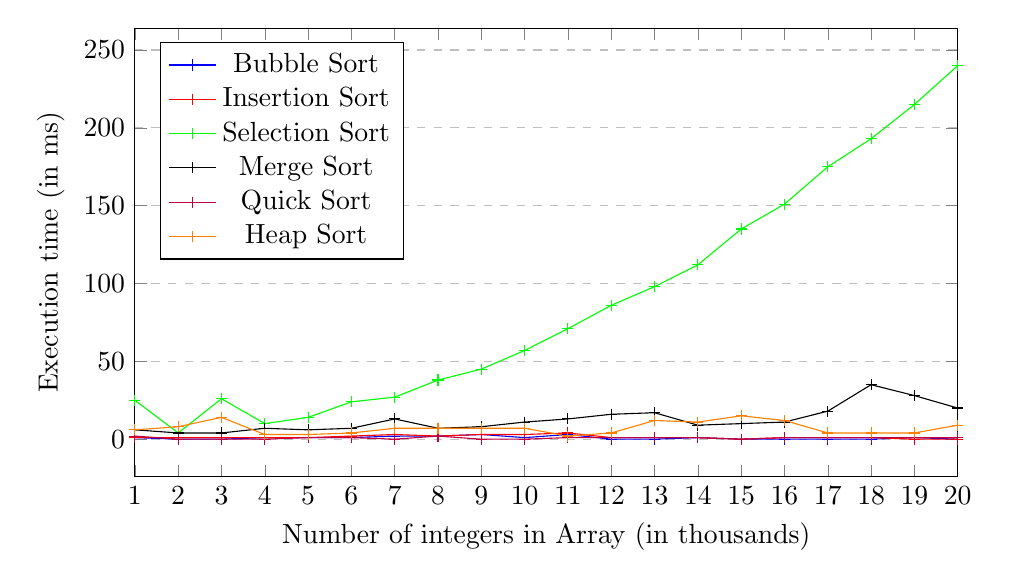
\begin{tikzpicture}
		\begin{axis}[
			xlabel={Number of integers in Array (in thousands)},
			ylabel={Execution time (in ms)},
			x=0.55cm,
			xmin=1, xmax=20,
			xtick={1, 2, 3, 4, 5, 6, 7, 8, 9, 10, 11, 12, 13, 14, 15, 16, 17, 18, 19, 20},
			ymajorgrids=true,
			grid style=dashed,
			legend pos=north west
			]
			
			\addplot[
			color=blue,
			mark=+,
			] 
			coordinates { (1,1)(2,0)(3,0)(4,1)(5,1)(6,1)(7,2)(8,2)(9,3)(10,1)(11,3)(12,0)(13,0)(14,1)(15,0)(16,0)(17,0)(18,0)(19,1)(20,0)};
			
			\addplot[
			color=red,
			mark=+,
			] 
			coordinates { (1,1)(2,1)(3,1)(4,1)(5,1)(6,2)(7,3)(8,2)(9,3)(10,3)(11,4)(12,1)(13,1)(14,1)(15,0)(16,1)(17,1)(18,1)(19,0)(20,0)};
			
			\addplot[
			color=green,
			mark=+,
			] 
			coordinates { (1,25)(2,4)(3,26)(4,10)(5,14)(6,24)(7,27)(8,38)(9,45)(10,57)(11,71)(12,86)(13,98)(14,112)(15,135)(16,151)(17,175)(18,193)(19,215)(20,240)};
			
			\addplot[
			color=black,
			mark=+,
			] 
			coordinates { (1,6)(2,4)(3,4)(4,7)(5,6)(6,7)(7,13)(8,7)(9,8)(10,11)(11,13)(12,16)(13,17)(14,9)(15,10)(16,11)(17,18)(18,35)(19,28)(20,20)};
			
			\addplot[
			color=purple,
			mark=+,
			] 
			coordinates { (1,2)(2,0)(3,0)(4,0)(5,1)(6,1)(7,0)(8,2)(9,0)(10,0)(11,1)(12,1)(13,1)(14,1)(15,0)(16,1)(17,1)(18,1)(19,1)(20,1)};
			
			\addplot[
			color=orange,
			mark=+,
			] 
			coordinates { (1,6)(2,8)(3,14)(4,3)(5,3)(6,4)(7,7)(8,7)(9,7)(10,7)(11,2)(12,4)(13,12)(14,11)(15,15)(16,12)(17,4)(18,4)(19,4)(20,9)};
			\legend{Bubble Sort, Insertion Sort, Selection Sort, Merge Sort, Quick Sort, Heap Sort}
		\end{axis}
	\end{tikzpicture}
	\caption{Execution time of the sorting algorithms with random ascending numbers}
	\label{ascFig}
\end{figure}

\subsubsection{Random Descending Integers}
Turning to the opposite of the previous special input, this section now considers a list of numbers sorted in descending order. Figure \ref{descFig} compares the different sorting algorithms runtime when dealing with random decreasing numbers. It can be seen in the figure that Bubble Sort performed faster than Selection Sort for most of the inputs, while Merge Sort, Quick Sort, and Heap Sort continues to be vastly faster than the other sorting algorithms.
\begin{figure}
	\centering
	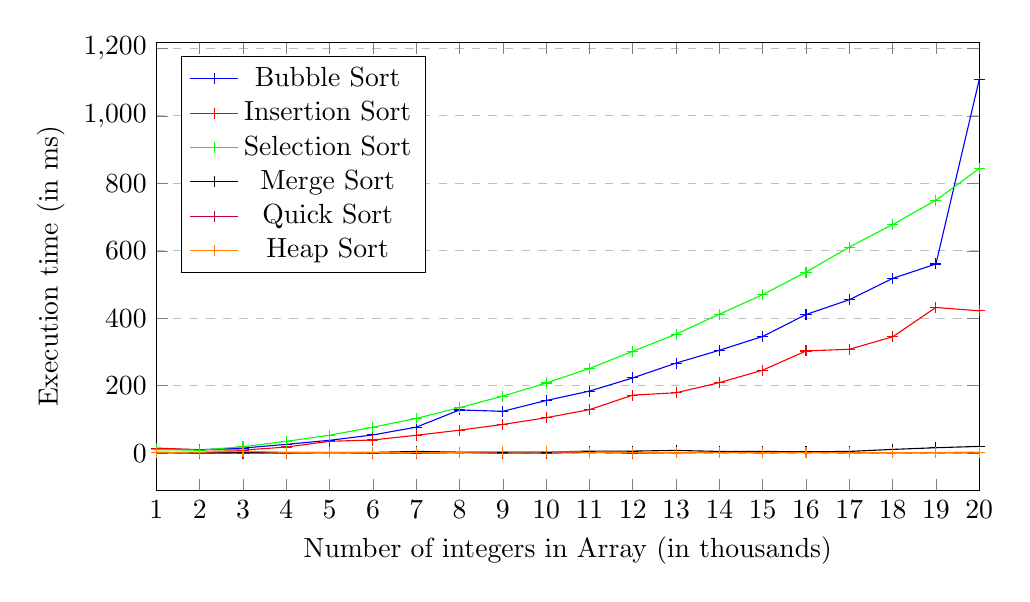
\begin{tikzpicture}
		\begin{axis}[
			xlabel={Number of integers in Array (in thousands)},
			ylabel={Execution time (in ms)},
			x=0.55cm,
			xmin=1, xmax=20,
			xtick={1, 2, 3, 4, 5, 6, 7, 8, 9, 10, 11, 12, 13, 14, 15, 16, 17, 18, 19, 20},
			ymajorgrids=true,
			grid style=dashed,
			legend pos=north west
			]
			
			\addplot[
			color=blue,
			mark=+,
			] 
			coordinates { (1,13)(2,10)(3,15)(4,26)(5,38)(6,54)(7,77)(8,128)(9,124)(10,156)(11,184)(12,223)(13,267)(14,305)(15,346)(16,411)(17,455)(18,518)(19,561)(20,1108)};
			
			\addplot[
			color=red,
			mark=+,
			] 
			coordinates { (1,15)(2,10)(3,9)(4,18)(5,35)(6,39)(7,53)(8,68)(9,85)(10,105)(11,129)(12,172)(13,179)(14,209)(15,246)(16,303)(17,308)(18,345)(19,432)(20,422)};
			
			\addplot[
			color=green,
			mark=+,
			] 
			coordinates { (1,10)(2,9)(3,19)(4,35)(5,53)(6,77)(7,103)(8,135)(9,169)(10,208)(11,251)(12,302)(13,353)(14,412)(15,470)(16,537)(17,611)(18,678)(19,750)(20,844)};
			
			\addplot[
			color=black,
			mark=+,
			] 
			coordinates { (1,2)(2,1)(3,1)(4,2)(5,2)(6,2)(7,5)(8,3)(9,3)(10,3)(11,6)(12,6)(13,8)(14,5)(15,5)(16,4)(17,5)(18,11)(19,16)(20,20)};
			
			\addplot[
			color=purple,
			mark=+,
			] 
			coordinates { (1,1)(2,0)(3,0)(4,0)(5,1)(6,0)(7,0)(8,1)(9,0)(10,0)(11,2)(12,0)(13,1)(14,2)(15,1)(16,2)(17,1)(18,1)(19,1)(20,1)};
			
			\addplot[
			color=orange,
			mark=+,
			] 
			coordinates { (1,2)(2,3)(3,6)(4,2)(5,1)(6,2)(7,1)(8,3)(9,4)(10,4)(11,3)(12,1)(13,1)(14,2)(15,2)(16,2)(17,2)(18,1)(19,2)(20,3)};
			\legend{Bubble Sort, Insertion Sort, Selection Sort, Merge Sort, Quick Sort, Heap Sort}
		\end{axis}
	\end{tikzpicture}
	\caption{Execution time of the sorting algorithms with random descending numbers}
	\label{descFig}
\end{figure}

\subsubsection{Random Restricted Integers}
Finally, this section focuses on the input where the numbers are bounded, ensuring the occurrence duplicates integers in the list. Figure \ref{restFig} displays the runtime of these algorithms working with the inputs. Despite the figure looking very similar to some other inputs, the runtime for each algorithm have been reduced significantly. However, Bubble Sort still performs the worst out of the 4 algorithms, having its runtime at large inputs nearly quadrupled that of the second worst algorithm, Insertion Sort.
\begin{figure}
	\centering
	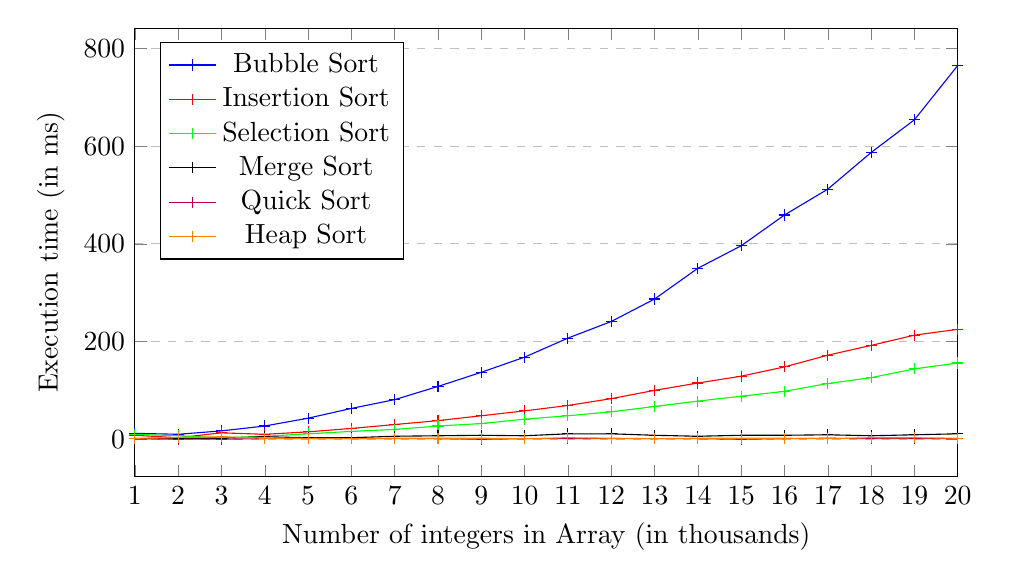
\begin{tikzpicture}
		\begin{axis}[
			xlabel={Number of integers in Array (in thousands)},
			ylabel={Execution time (in ms)},
			x=0.55cm,
			xmin=1, xmax=20,
			xtick={1, 2, 3, 4, 5, 6, 7, 8, 9, 10, 11, 12, 13, 14, 15, 16, 17, 18, 19, 20},
			ymajorgrids=true,
			grid style=dashed,
			legend pos=north west
			]
			
			\addplot[
			color=blue,
			mark=+,
			] 
			coordinates { (1,12)(2,10)(3,17)(4,27)(5,43)(6,63)(7,81)(8,108)(9,137)(10,168)(11,207)(12,241)(13,287)(14,350)(15,396)(16,459)(17,512)(18,587)(19,654)(20,765)};
			
			\addplot[
			color=red,
			mark=+,
			] 
			coordinates { (1,8)(2,3)(3,13)(4,10)(5,15)(6,22)(7,30)(8,38)(9,48)(10,58)(11,69)(12,83)(13,100)(14,115)(15,129)(16,148)(17,172)(18,192)(19,213)(20,225)};
			
			\addplot[
			color=green,
			mark=+,
			] 
			coordinates { (1,10)(2,7)(3,3)(4,6)(5,11)(6,16)(7,20)(8,27)(9,32)(10,41)(11,48)(12,56)(13,67)(14,78)(15,88)(16,98)(17,114)(18,126)(19,144)(20,156)};
			
			\addplot[
			color=black,
			mark=+,
			] 
			coordinates { (1,1)(2,2)(3,2)(4,5)(5,3)(6,3)(7,6)(8,7)(9,8)(10,7)(11,11)(12,11)(13,8)(14,6)(15,8)(16,8)(17,9)(18,7)(19,9)(20,11)};
			
			\addplot[
			color=purple,
			mark=+,
			] 
			coordinates { (1,1)(2,0)(3,0)(4,1)(5,1)(6,1)(7,1)(8,1)(9,0)(10,1)(11,1)(12,1)(13,1)(14,1)(15,0)(16,1)(17,2)(18,1)(19,1)(20,1)};
			
			\addplot[
			color=orange,
			mark=+,
			] 
			coordinates { (1,2)(2,3)(3,5)(4,2)(5,2)(6,1)(7,2)(8,2)(9,2)(10,1)(11,3)(12,2)(13,1)(14,2)(15,2)(16,2)(17,1)(18,3)(19,3)(20,2)};
			\legend{Bubble Sort, Insertion Sort, Selection Sort, Merge Sort, Quick Sort, Heap Sort}
		\end{axis}
	\end{tikzpicture}
	\caption{Execution time of the sorting algorithms with random numbers between 1 (inclusive) and 100 (exclusive)}
	\label{restFig}
\end{figure}

\subsection{Memory Usage}
To answer the third experiment aim, we will utilize the algorithm as detailed in the Experimental Setup and Procedure section. Table \ref{memArr} shows the maximum array size given the maximum heap size allocated for the Java Virtual Machine is four megabytes. From the graph, it can be seen that Merge Sort used the most memory, only just managing an array of 40 thousand. Meanwhile, Bubble Sort, Selection Sort, and Heap Sort used the least amount of memory, sorting arrays at the maximum size of 130 thousand.

\begin{figure}
	\centering
	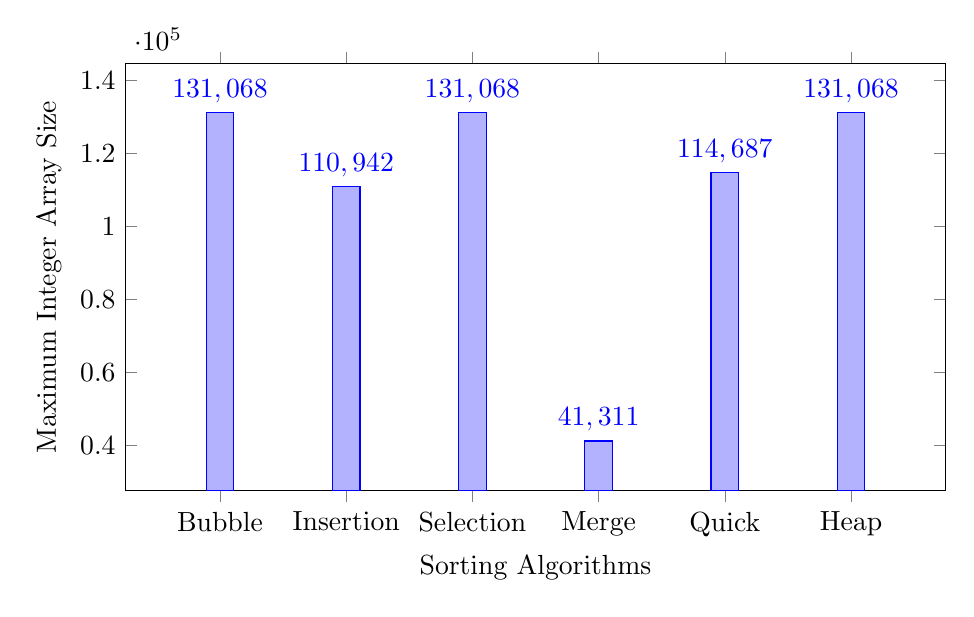
\begin{tikzpicture}
		\begin{axis}
			[
				ybar,
				width=12cm,
				height=7cm,
				xlabel=Sorting Algorithms,
				symbolic x coords={Bubble, Insertion, Selection, Merge, Quick, Heap},
				xtick=data,
				ylabel=Maximum Integer Array Size,
				enlargelimits=0.15,
				nodes near coords,
				every node near coord/.append style={/pgf/number format/.cd, fixed,1000 sep={,}}
			]
			
			\addplot coordinates {
				(Bubble, 131068) (Insertion, 110942) (Selection, 131068) (Merge, 41311) (Quick, 114687) (Heap, 131068)
			};
		\end{axis}
	\end{tikzpicture}
	\caption{Maximum array length for each sorting algorithm with maximum heap size of 4 megabytes}
	\label{memArr}
\end{figure}

\section{Discussion}
After presenting the results, this section will reflect on the findings and come up with plausible explanations for why it does or does not match with the hypothesis. This section will discuss the performance of algorithms with respect to time under random integer arrays of small and big sizes, time under special random integer arrays, and the memory usage of each algorithm.

\subsection{Execution Time of Random Integer Arrays of Varied Size}
As expected from Figure \ref{bigFig}, Bubble Sort, Insertion Sort, and Selection Sort all have the same growth rate, albeit some grew faster than others. This lines up with our hypothesis, as the time complexity of those 3 algorithms grows quicker than the time complexity of Merge Sort, Quick Sort, and Heap Sort in the average-case. Although, when dealing with smaller inputs, the results tend to vary themselves in a more chaotic manner than the bigger inputs, as can be seen in Figure \ref{smallFig}. This is also expected, as asymptotic notation only bounds after a large enough input, as given by the formal definitions in the introduction section. Similar results were also found in Karunanithi's own investigation into the performance of sorting algorithms \autocite{karunanithi2014survey}.

\subsection{Execution Time of Special Random Integer Arrays}
The purpose of this section is to look at the performance when given the best and worst-case inputs. Observing the graph in Figure \ref{ascFig}, it is clear that there were massive improvements for Bubble Sort and Insertion Sort. Indeed, Bubble Sort would only swap if there still are elements out-of-order, which is not the case with an already sorted array of numbers. Similarly, Insertion Sort checks from the last sorted array index, which is always smaller than the current index its comparing to in a sorted array. Hence, the insanely fast speeds that Bubble Sort and Insertion Sort reached, which is $O(n)$ as only one pass of the array was needed.

Surprisingly, while Quick Sort was hypothesized to perform the worst when the array is already sorted in either ascending or descending order, it still outperformed every other algorithm no matter the input. This is caused by the implementation of Quick Sort, in that the chosen pivot was not the first nor last element, but the middle element, as specified for the implementation of "Fat Partitioning". This led to the list division being a perfect even split, thus contributing no extra time.

When confronted with integer arrays with multiple repeated elements, the performance showed little to no difference to the one with random integer arrays. This suggests that the element values itself has no importance when it comes to sorting, other than comparison. However, this experiment is treating all integers are the same, that is, an integer is indistinguishable from another integer with the same value. If one wishes to sort an array and keep the same order if duplicated values arise, then certain algorithms will not be applicable for these kinds of tasks. This is not a focus on the experiment, however it is important to notice when taking into consideration what sorting algorithms to implement for a project.

\subsection{Memory Usage of Sorting Algorithms}
Finally, exploring the topic of memory usage, this experiment also set out to compute the maximum length of an array before an out of memory exception was thrown. Insertion Sort and Quick Sort returned slightly worse array lengths than the expected, possibly due to the amount of variables, miscellaneous helper functions, or function calls for code organization. However, Merge Sort performed the worst out of the 6 algorithms, which is what was expected, considering its memory complexity was the only one in linear usage $O(n)$. Indeed, Merge Sort is not an in-place algorithm, meaning it creates a new list with the sorted items rather than modifying its input array, hence the lower maximum array length.

Identical results can also be seen from Karunanithi's investigation too, where the findings he came up with showed that every sorting algorithm used the same amount of memory space, other than Merge Sort, which had close to double the memory consumption than the rest \autocite{karunanithi2014survey}.

\section{Conclusion}
This report has explored the performance of 6 sorting algorithms in a variety of different inputs. The time and memory performance of which was recorded in graphs for meaningful discussions and interpretations of the data. Furthermore, it was also discussed the common methods of measuring algorithmic efficiency with the asymptotic notation and worst-case analysis.

Although this report has tried to be as comprehensive as possible, there are still areas where this report failed at. The maximum input array experiment had to have limited maximum memory heap of four megabytes for the Java Virtual Machine, as the default, which is less than one-fourth of the total available physical memory \autocite{ParallelCollector}, would take too long to compute for each search iteration. For future research opportunities, a different approach to calculating the memory usage can be taken, although it could be considered a challenge due to how non-deterministic memory allocation on a machine can be.

This report is beneficial for prospective computer science students to introduce them to the world of algorithmic thinking and optimizations. Sorting algorithms are simple procedures, yet have incredible depth as to what approaches can be taken to solve the problem, as well as techniques to analyze theoretical performance of an algorithm. Through this report, the hope is that an understanding regarding computational complexity can be reached.

\printbibliography

\end{document}